%%%%%%%%%%%%%%%%%%%%%%%%%%%%%%%%%%%%%%%%%%%%%%%%%%%%%%%%%%%%%%%%%%%%%%%%%%%%%
%  enslyonreview.tex — Guide d'utilisation de la classe enslyonreview v1.1
%
%  Compilez avec : pdflatex enslyonreview → biber enslyonreview → pdflatex ×2
%%%%%%%%%%%%%%%%%%%%%%%%%%%%%%%%%%%%%%%%%%%%%%%%%%%%%%%%%%%%%%%%%%%%%%%%%%%%%

\documentclass[11pt, a4paper]{article}

% ── Encodage et langue ─────────────────────────────────────────────────────
\usepackage[utf8]{inputenc}
\usepackage[T1]{fontenc}
\usepackage[french]{babel}
% French babel makes ":" an "active" shorthand character (for the thin
% space it inserts before colons) — this breaks cleveref's internal
% \csname-building for any label containing a colon, e.g. \label{sec:foo},
% with a cryptic "Missing \endcsname inserted" error. Disabling just the
% ":" shorthand is the standard, documented fix — done at \begin{document}
% since babel re-enables its shorthands there, after the preamble runs.
\AtBeginDocument{\shorthandoff{:}}
\usepackage{csquotes}
\usepackage{newtxtext}
\usepackage{newtxmath}

% siunitx + mhchem — loaded here (not just described) so the demo in
% "Unités et formules chimiques" actually executes \qty/\unit/\ce, rather
% than showing hand-typed fake output next to the code.
\usepackage{siunitx}
\usepackage[version=4]{mhchem}
% Molar ("M", mol/L) isn't a real SI unit, so siunitx v3 doesn't know it
% out of the box — \DeclareSIUnit is the documented, non-hacky way to add
% it (rather than hand-rolling a \newcommand), exactly as recommended for
% this kind of unit.
\DeclareSIUnit{\Molar}{M}

% ── Géométrie ──────────────────────────────────────────────────────────────
\usepackage[margin=25mm, headheight=15pt]{geometry}

% ── Couleurs (palette officielle enslyonreview : rouille / pêche) ─────────
\usepackage{xcolor}
\definecolor{darkbg}     {HTML}{F5EFE7}
\definecolor{codegray}   {HTML}{2C1E14}
\definecolor{codepurple} {HTML}{7B2F8B}
\definecolor{codeblue}   {HTML}{B74600}
\definecolor{codegreen}  {HTML}{2E7D32}
\definecolor{codecomment}{HTML}{8B7355}
\definecolor{ENSorange}  {HTML}{B74600}
\definecolor{ENSaccent}  {HTML}{E07820}
\definecolor{ENSbg}      {HTML}{FFF3E9}
\definecolor{ENSmeta}    {HTML}{FFCC99}
\definecolor{ENSabstract}{HTML}{E6E6E6}
\definecolor{tipsblue}   {HTML}{1A5C9E}
\definecolor{tipsbg}     {HTML}{EDF4FB}
\definecolor{warnred}    {HTML}{A62020}
\definecolor{warnbg}     {HTML}{FBF0F0}
\definecolor{resultbg}   {HTML}{FFFFFF}

% ── Coloration syntaxique des exemples de code ─────────────────────────────
\usepackage{listings}
\lstdefinestyle{latexcode}{
  language=[LaTeX]TeX,
  backgroundcolor=\color{darkbg},
  basicstyle=\ttfamily\small\color{codegray},
  keywordstyle=\color{codepurple}\bfseries,
  commentstyle=\color{codecomment}\itshape,
  stringstyle=\color{codegreen},
  breaklines=true,
  breakatwhitespace=false,
  tabsize=2,
  showstringspaces=false,
  columns=flexible,
  keepspaces=true,
  frame=none,
  numbers=none,
  aboveskip=0pt,
  belowskip=0pt,
  literate=
    {à}{{\`a}}1 {â}{{\^a}}1 {ä}{{\"a}}1
    {é}{{\'e}}1 {è}{{\`e}}1 {ê}{{\^e}}1 {ë}{{\"e}}1
    {î}{{\^i}}1 {ï}{{\"i}}1 {í}{{\'i}}1
    {ô}{{\^o}}1 {ö}{{\"o}}1 {ó}{{\'o}}1
    {ù}{{\`u}}1 {û}{{\^u}}1 {ü}{{\"u}}1 {ú}{{\'u}}1
    {ç}{{\c c}}1 {œ}{{\oe{}}}1 {æ}{{\ae}}1 {ñ}{{\~n}}1
    {É}{{\'E}}1 {È}{{\`E}}1 {Ê}{{\^E}}1 {Í}{{\'I}}1
    {À}{{\`A}}1 {Â}{{\^A}}1 {Ó}{{\'O}}1
    {Ô}{{\^O}}1 {Ç}{{\c C}}1 {Ú}{{\'U}}1 {Ñ}{{\~N}}1
    {—}{{---}}1 {–}{{--}}1 {°}{{$^\circ$}}1
    {•}{{$\bullet$}}1,
  morekeywords={[2]reviewtitle,reviewshorttitle,reviewauthor,reviewauthorshort,
    reviewaffiliation,reviewdate,reviewkeywords,reviewabstract,maketitle,
    addbibresource,cite,printbibliography,refspecialinterest,
    refoutstandinginterest,cref,Cref,label,reviewnote,reviewbox,
    documentclass,section,subsection,noreflegend,bibref,bibdoi,bibpmid,
    bibpmcid,ofspecialinterest,ofoutstandinginterest,references,item},
  keywordstyle={[2]\color{codeblue}\bfseries},
}

% ── tcolorbox : bloc "code + résultat" et encadrés astuce/attention ───────
\usepackage{tcolorbox}
\tcbuselibrary{listings, skins, breakable, most}
\usepackage{changepage}

\newtcolorbox{demoinner}[1][]{
  enhanced, sidebyside, sidebyside align=center seam,
  lefthand width=\dimexpr3\linewidth/5-3mm\relax,
  sidebyside gap=3mm,
  colback=darkbg, colbacklower=resultbg, colframe=ENSorange!80,
  left=2pt, right=2pt, top=4pt, bottom=4pt,
  fonttitle=\sffamily\bfseries\small,
  #1
}
\NewDocumentEnvironment{demo}{O{}}{%
  \begin{adjustwidth}{-14mm}{-14mm}\noindent\begin{demoinner}[#1]%
}{%
  \end{demoinner}\end{adjustwidth}%
}

\newtcolorbox{astuce}{
  enhanced, colback=tipsbg, colframe=tipsblue,
  leftrule=4pt, rightrule=0.4pt, toprule=0.4pt, bottomrule=0.4pt,
  arc=2pt, left=8pt, fonttitle=\sffamily\bfseries\color{tipsblue},
  title={Astuce}, attach title to upper={\ —\ },
}
\newtcolorbox{attention}{
  enhanced, colback=warnbg, colframe=warnred,
  leftrule=4pt, rightrule=0.4pt, toprule=0.4pt, bottomrule=0.4pt,
  arc=2pt, left=8pt, fonttitle=\sffamily\bfseries\color{warnred},
  title={Attention}, attach title to upper={\ —\ },
}

% ── Simulation de l'apparence enslyonreview dans la colonne "résultat" ────
\newcommand{\simcite}[1]{\textcolor{ENSorange}{\bfseries[#1]}}
\newcommand{\simsection}[1]{%
  \colorbox{white}{\parbox{\dimexpr\linewidth-2\fboxsep\relax}{%
    \color{ENSorange}\bfseries\normalsize #1}}\par}
\newcommand{\simmeta}[1]{%
  \noindent\colorbox{ENSmeta}{\parbox{\dimexpr\linewidth-2\fboxsep\relax}{\small #1}}\par}
\newcommand{\simabstract}[1]{%
  \noindent\colorbox{ENSabstract}{\parbox{\dimexpr\linewidth-2\fboxsep\relax}{\small\bfseries #1}}\par}
\newcommand{\simbar}[1]{%
  \noindent\colorbox{ENSorange}{\parbox{\dimexpr\linewidth-2\fboxsep\relax}{\small\color{white} #1}}\par}
% Lien (rendu de \crefcolor/\Crefcolor — coloré ET gras)
\newcommand{\simlinkbold}[1]{\textbf{\textcolor{ENSorange}{#1}}}

% Rendu du texte dans une vraie police (texte seul, pas les maths — évite
% de charger plusieurs packages de maths concurrents dans le même
% document, ce qui casserait les symboles) — \infont{code NFSS}{texte}
\newcommand{\infont}[2]{{\fontfamily{#1}\selectfont #2}}

% Nuancier de thème : pastille de couleur + nom — \sw{RRGGBB}{nom}
\newcommand{\sw}[2]{%
  \colorbox[HTML]{#1}{\rule{0pt}{5.5pt}\hspace{9pt}}~\textbf{\small #2}}

% Placeholder de figure avec légende, imitant \includegraphics + \caption
% dans une figure/figure* — \simfigbox[nom-de-fichier]{texte de légende}
\newcommand{\simfigbox}[2][fig.pdf]{%
  \begin{center}
    \fbox{\parbox{0.8\linewidth}{\centering\vspace{8pt}%
      \textcolor{gray!60}{\rule{2.4cm}{1.5cm}}\\[4pt]
      {\tiny\ttfamily\color{gray} #1}\vspace{8pt}}}\\[4pt]
    {\small\textcolor{ENSorange}{\textbf{Figure~1.}}\ #2}%
  \end{center}}

% Encadré "Box N." imitant le flottant reviewbox (floatstyle=boxed) — la
% légende est HORS de l'encadré, au-dessus (comportement réel de la
% classe : \@fs@iftopcapt), pas à l'intérieur — \simbox{numéro}{titre}{contenu}
\newcommand{\simbox}[3]{%
  {\small\textbf{\textcolor{ENSorange}{Box #1.}}~\textbf{#2}}\\[4pt]
  \noindent\fcolorbox{ENSorange}{white}{\parbox{\dimexpr\linewidth-2\fboxsep-2\fboxrule\relax}{%
    \vspace{2pt}\small #3\vspace{2pt}}}}

% ── Hyperliens, en-têtes, mise en page ─────────────────────────────────────
\usepackage[colorlinks, linkcolor=ENSorange, urlcolor=ENSaccent,
            citecolor=ENSorange, pdftitle={Guide enslyonreview},
            pdfauthor={Adama Mbaye}]{hyperref}
\usepackage{cleveref}
\usepackage{fancyhdr}
\pagestyle{fancy}
\fancyhf{}
\fancyhead[L]{\small\sffamily\color{ENSorange} Guide \texttt{enslyonreview} v1.1}
\fancyhead[R]{\small\sffamily\leftmark}
\fancyfoot[C]{\small\sffamily\thepage}
\renewcommand{\headrulewidth}{0.4pt}
\renewcommand{\headrule}{{\color{ENSorange}\hrule width\headwidth height 0.4pt}}

\usepackage{graphicx}
\graphicspath{{figures/}}
\usepackage{booktabs}
\usepackage{enumitem}
\usepackage{microtype}
\usepackage{lastpage}
\setcounter{tocdepth}{2}

\usepackage{titlesec}
\titleformat{\section}{\color{ENSorange}\Large\bfseries}{\thesection.}{0.5em}{}
  [\color{ENSorange}\rule{\linewidth}{0.6pt}]
\titleformat{\subsection}{\color{ENSorange}\large\bfseries}{\thesubsection}{0.5em}{}
\titleformat{\subsubsection}{\bfseries}{\thesubsubsection}{0.5em}{}

\newcommand{\BibTeX}{\textsc{Bib}\TeX}

\begin{document}

% ═══════════════════════════════════════════════════════════════════════════
\begin{titlepage}
\centering
\vspace*{2cm}
{\Huge\bfseries\color{ENSorange} enslyonreview}\\[8pt]
{\Large Classe \LaTeX{} pour la revue bibliographique M2 Biosciences}\\[4pt]
{\large (format Current Opinion)}\\[2cm]

\colorbox{ENSmeta}{\parbox{0.7\linewidth}{\centering\vspace{4pt}
  \textbf{Guide d'utilisation} — version 1.1 (septembre 2026)\\
  École Normale Supérieure de Lyon — Département de Biologie\\
  UE Analyse bibliographique M2 Biosciences\vspace{4pt}}}

\vspace{2cm}
Reproduit en \LaTeX{} le template LibreOffice \texttt{review\_M2.ott}
fourni par F.~Roudier, responsable de l'UE. Package frère de
\texttt{enslyonstage} (rapports de stage M1/M2).

\vspace{1.5cm}
\begin{tcolorbox}[colback=darkbg, colframe=ENSorange!40, width=0.85\linewidth,
                   left=8pt, right=8pt]
\small\sffamily
Ce guide explique toutes les commandes de la classe. Chaque encadré
présente le \textbf{code} à écrire à gauche et le \textbf{rendu visuel}
correspondant à droite. Pour un document complet compilé, ouvrez
\texttt{enslyonreview-exemple.tex} (ou son PDF, fourni à côté).
\end{tcolorbox}

\vfill
{\small Auteur : Adama \textsc{Mbaye} \quad|\quad Licence : LPPL 1.3c}
\end{titlepage}

\tableofcontents
\clearpage

% ═══════════════════════════════════════════════════════════════════════════
\section{Introduction}
\label{sec:intro}
% ═══════════════════════════════════════════════════════════════════════════

\texttt{enslyonreview} est une classe \LaTeX{} qui reproduit la mise en
forme exigée pour la revue bibliographique de M2 Biosciences (UE
``Analyse bibliographique'', responsable F.~Roudier) : format à l'imitation
des revues \emph{Current Opinion}, bloc de titre avec résumé et mots-clés,
deux colonnes, en-tête/pied de page avec pagination, figures/tableaux/box,
et une bibliographie numérotée avec annotations ``of special/outstanding
interest''.

Le template officiel de référence est le fichier LibreOffice
\texttt{review\_M2.ott} distribué par F.~Roudier ; \texttt{enslyonreview}
en est une traduction fidèle en \LaTeX{}, avec en plus une bibliographie
réellement fonctionnelle (citations cliquables, numérotées et compilées
automatiquement depuis un fichier \texttt{.bib}, au lieu de texte
tapé à la main).

\subsection{Fichiers du package}

\begin{center}
\small
\begin{tabular}{@{}ll@{}}
\toprule
\textbf{Fichier} & \textbf{Rôle} \\
\midrule
\texttt{enslyonreview.cls} & La classe elle-même \\
\texttt{enslyonreview.dbx} & Champs bibliographiques personnalisés (pmid, pmcid\ldots) \\
\texttt{enslyonreview-gabarit.tex} & Modèle vierge — à copier pour démarrer \\
\texttt{references.bib} & Base bibliographique vierge, pour le gabarit \\
\texttt{enslyonreview-exemple.tex} & Exemple entièrement rédigé \\
\texttt{enslyonreview-exemple.bib} & Les 50 références de l'exemple \\
\texttt{enslyonreview.tex} / \texttt{.pdf} & Ce guide \\
\texttt{README.md} & Instructions rapides (version courte de ce guide) \\
\texttt{LICENSE} & LPPL 1.3c \\
\bottomrule
\end{tabular}
\end{center}

\subsection{Exigences de l'UE}

D'après les consignes officielles de F.~Roudier (cohorte 2025–2026) :

\begin{center}
\small
\begin{tabular}{@{}ll@{}}
\toprule
\textbf{Critère} & \textbf{Valeur} \\
\midrule
Références & 30 à 50 \\
Longueur & \textasciitilde 25\,000 caractères \\
Figures/tableaux & 3 à 5 \\
Sujet & lié à votre stage, mais plus large ; non redondant \\
 & avec l'introduction du rapport de stage \\
Format & compatible \emph{Current Opinion} (ce que reproduit la classe) \\
Rendu & PDF, déposé sur le Portail \\
\bottomrule
\end{tabular}
\end{center}

\begin{attention}
Chiffres de la cohorte \textbf{2025--2026}, susceptibles de changer d'une
année sur l'autre (notamment les dates de rendu) — vérifiez-les auprès de
F.~Roudier pour votre propre promotion avant de rendre votre revue.
\end{attention}

% ═══════════════════════════════════════════════════════════════════════════
\section{Démarrage rapide}
\label{sec:quickstart}
% ═══════════════════════════════════════════════════════════════════════════

\begin{enumerate}
  \item \textbf{Overleaf~:} téléversez tous les fichiers du package (y
    compris \texttt{.cls} et \texttt{.dbx}, ainsi que le dossier
    \texttt{figures/}). Overleaf détecte \texttt{enslyonreview-gabarit.tex}
    comme fichier racine et lance \texttt{biber} automatiquement.
  \item \textbf{Remplissez les métadonnées} dans le préambule de
    \texttt{enslyonreview-gabarit.tex} (\cref{sec:titlepage}).
  \item \textbf{Ajoutez vos références} dans \texttt{references.bib}
    (\cref{sec:biblio}) et vos figures dans \texttt{figures/}.
  \item \textbf{Écrivez vos sections} en vous inspirant de ce guide ou de
    \texttt{enslyonreview-exemple.tex}.
  \item \textbf{Compilez} avec pdf\LaTeX{} + biber
    (\cref{sec:compilation}) — automatique à chaque sauvegarde sur
    Overleaf.
\end{enumerate}

Point de départ concret — le squelette minimal d'un document
\texttt{enslyonreview} :

\begin{lstlisting}[style=latexcode]
\documentclass{enslyonreview}


\reviewtitle{Votre titre}
\reviewshorttitle{Titre court}

\reviewauthor{Prénom \textsc{Nom}}
\reviewauthorshort{Nom}

\reviewaffiliation{Master BioSciences, Département de Biologie, École Normale 
	Supérieure de Lyon.}
	
\reviewdate{2027-01-15}

\reviewkeywords{mot-clé1, mot-clé2, mot-clé3}

\reviewabstract{Votre résumé, en un seul paragraphe.}

\addbibresource{references.bib}

\begin{document}
\maketitle

\section{Introduction}
Votre texte, avec des citations \cite{maCle2024}\ldots

\printbibliography[title=References]
\end{document}
\end{lstlisting}

% ═══════════════════════════════════════════════════════════════════════════
\section{Page de titre}
\label{sec:titlepage}
% ═══════════════════════════════════════════════════════════════════════════

Toutes les métadonnées se déclarent dans le \emph{préambule}, avant
\verb|\begin{document}|, puis \verb|\maketitle| assemble le bloc de titre
(sur toute la largeur de la page, avant que le document ne bascule en deux
colonnes pour le corps du texte).

\subsection{\texttt{\textbackslash reviewtitle\{\}} et \textbackslash reviewshorttitle\{\}}

\begin{demo}
\begin{lstlisting}[style=latexcode]
\reviewtitle{Antiviral restriction factors in immunity and disease}

\reviewshorttitle{Antiviral Restriction Factors}
\end{lstlisting}
\tcblower
{\bfseries\color{ENSorange}\large Antiviral restriction factors in
immunity and disease}\\[6pt]
{\footnotesize\itshape Le titre complet s'affiche en haut de la page 1 ;
le titre court apparaît dans le bandeau d'en-tête de chaque page.}
\end{demo}

\newpage

\subsection{\texttt{\textbackslash reviewauthor\{\}}, \textbackslash reviewaffiliation\{\} et \textbackslash reviewdate\{\}}

Les trois s'affichent \textbf{ensemble} dans le même bandeau pêche sous le
titre — le nom en gras en première ligne, puis affiliation et date. Seul
\texttt{\textbackslash reviewauthorshort} (ci-dessous) en est indépendant :
il n'apparaît jamais dans ce bandeau, seulement dans l'en-tête de chaque page.

\begin{demo}
\begin{lstlisting}[style=latexcode]
\reviewauthor{Erika \textsc{Larrahondo Rodriguez}}
\reviewaffiliation{Master Biosciences,
  Departement de Biologie,
  \'Ecole Normale Superieure de Lyon.}
\reviewdate{Dec 2024}
\end{lstlisting}
\tcblower
\simmeta{\textbf{\large Erika \textsc{Larrahondo Rodríguez}}\\[2pt]
\textit{Master Biosciences, Département de Biologie, École Normale
Supérieure de Lyon.}\\[2pt] Dec 2024}
\vspace{1em}
{\footnotesize\itshape \texttt{\textbackslash textsc\{\}} met le nom de
famille en petites capitales (convention reprise d'\texttt{enslyonstage}).
La date réapparaît aussi, seule, dans le pied de page de chaque page.}
\end{demo}

\subsection{\texttt{\textbackslash reviewauthorshort\{\}}}

\begin{demo}
\begin{lstlisting}[style=latexcode]
\reviewauthorshort{Larrahondo Rodriguez}
\end{lstlisting}
\tcblower
{\footnotesize\itshape Le nom court (souvent juste le nom de famille, sans
petites capitales) apparaît en italique dans le bandeau d'en-tête de
chaque page, à côté du titre court — jamais dans le bandeau pêche de la
page 1.}
\end{demo}

\subsection{\texttt{\textbackslash reviewkeywords\{\}} et \textbackslash reviewabstract\{\}}

\begin{demo}
\begin{lstlisting}[style=latexcode]
\reviewkeywords{Antiviral, disease, innate immunity}

\reviewabstract{Antiviral factors from the cell autonomous innate immunity are essential cellular proteins\ldots}
\end{lstlisting}
\tcblower
\simabstract{Keywords: Antiviral, disease, innate immunity}
\vspace{4pt}
\simabstract{Antiviral factors from the cell autonomous innate
immunity are essential cellular proteins\ldots}
{\footnotesize\itshape Chacun dans son propre encadré grisé, l'un sous
l'autre.}
\end{demo}

\newpage

\subsection{Résultat~: rendu réel de la page 1}

Ces quatre commandes assemblées donnent, une fois compilées, le bloc de
titre pleine largeur reproduit ci-dessous — extrait tel quel de la page 1
de \texttt{enslyonreview-exemple.tex} :

\begin{center}
  \fbox{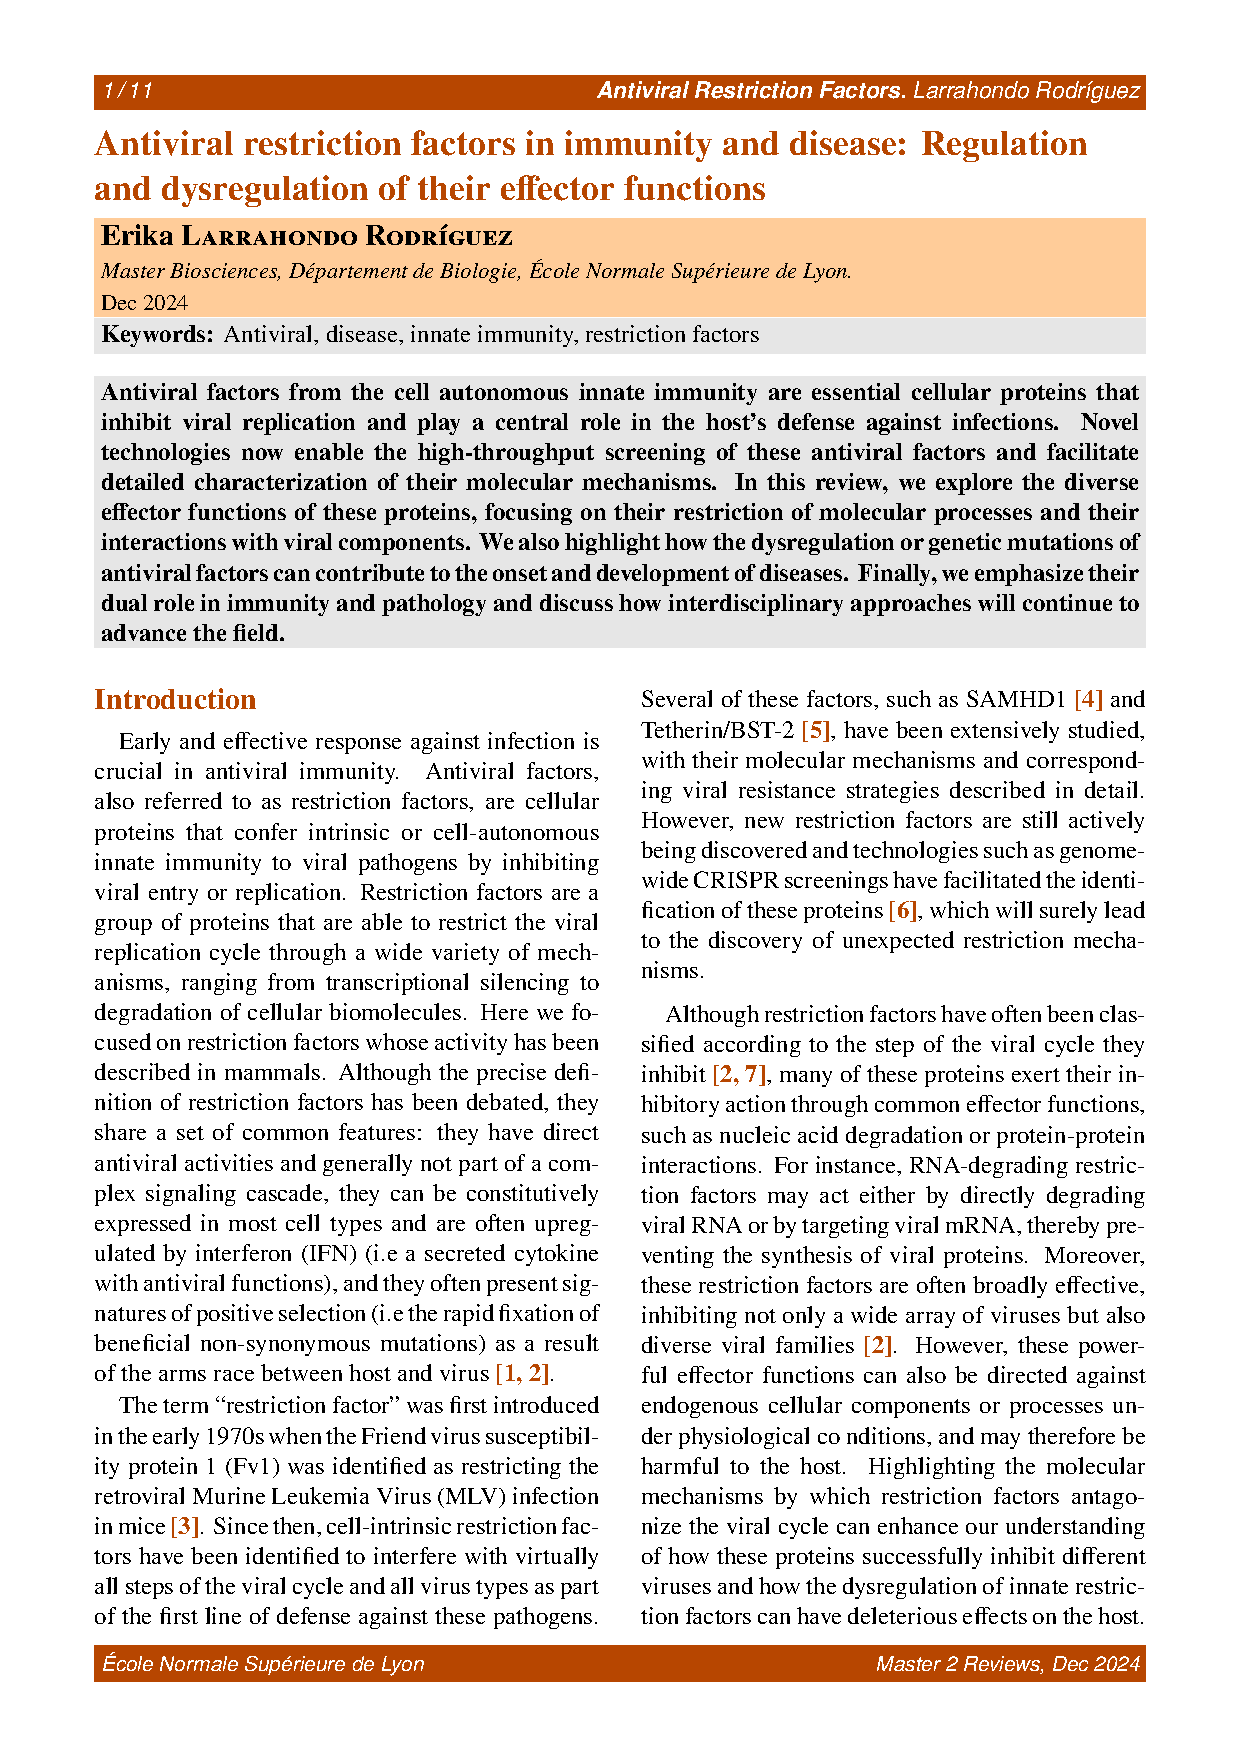
\includegraphics[page=1, width=0.62\linewidth]{enslyonreview-exemple.pdf}}\\[6pt]
  {\footnotesize\itshape Page 1 de \texttt{enslyonreview-exemple.tex} —
  thème \texttt{orange} (défaut).}
\end{center}

%\newpage

% ═══════════════════════════════════════════════════════════════════════════
\section{Thèmes et police}
\label{sec:themes}
% ═══════════════════════════════════════════════════════════════════════════

\subsection{Thèmes de couleur}

23 thèmes sont disponibles, comme dans \texttt{enslyonstage} (plus un).
Le thème \texttt{orange} (par défaut) reprend la charte rouille/pêche
officielle du \texttt{.ott} ; \texttt{orangeens} est l'orange
\emph{institutionnel} de l'ENS de Lyon (le même que le thème par défaut
d'\texttt{enslyonstage}) — différent de celui du \texttt{.ott}, pour qui
préfère la couleur école plutôt que celle du template. Les 21 autres sont
des variantes de confort si vous préférez une autre couleur dominante
pour vos propres essais.

\begin{demo}
\begin{lstlisting}[style=latexcode]
\documentclass{enslyonreview}
% orange (defaut, officiel .ott)

\documentclass[orangeens]{enslyonreview}
% orange institutionnel ENS de Lyon

\documentclass[blue]{enslyonreview}
% ou un autre theme nomme
\end{lstlisting}
\tcblower
\footnotesize
\begin{tabular}{@{}lll@{}}
  \sw{B74600}{orange}\,\textsuperscript{*} & \sw{E14D17}{orangeens}\,\textsuperscript{\dag} & \sw{652080}{violet} \\[3pt]
  \sw{1A5C9E}{blue}                         & \sw{A62020}{red}      & \sw{1E6B3A}{green}   \\[3pt]
  \sw{0E6B6B}{teal}                         & \sw{3A3A3A}{gray}     & \sw{0D3B6E}{navy}    \\[3pt]
  \sw{1D4ED8}{azure}                        & \sw{3730A3}{indigo}   & \sw{1E2D5C}{midnight}\\[3pt]
  \sw{334155}{slate}                        & \sw{5B21B6}{purple}   & \sw{9D174D}{pink}    \\[3pt]
  \sw{881337}{crimson}                      & \sw{63152D}{wine}     & \sw{92400E}{amber}   \\[3pt]
  \sw{7A5300}{gold}                         & \sw{5C2D0E}{brown}    & \sw{365314}{lime}    \\[3pt]
  \sw{14532D}{forest}                       & \sw{0E6B8E}{cyan}     &                      \\
\end{tabular}\\[4pt]
{\itshape\footnotesize\textsuperscript{*}orange — charte
rouille/pêche de \texttt{review\_M2.ott}. \textsuperscript{\dag}orange
institutionnel ENS de Lyon (identique au thème par défaut
d'\texttt{enslyonstage}). Chacun affecte titres, bandeaux, citations et
liens.}
\end{demo}

\begin{astuce}
Pour une remise officielle, gardez le thème \texttt{orange} par défaut —
c'est celui qui correspond à la charte du \texttt{.ott}.
\end{astuce}

\subsection{Police — options \texttt{[palatino]}, \texttt{[xcharter]}, \texttt{[stix]}}

Par défaut, le corps du texte utilise \texttt{newtx} (métriques Times New
Roman, fidèles au \texttt{.ott}). Trois options basculent tout le document
(texte \emph{et} maths) vers une autre police académique à la place —
chacune vérifiée avec de vraies petites capitales
(\texttt{\textbackslash textsc\{\}}, \cref{sec:titlepage}) \emph{et} de
vraies formules mathématiques (intégrales, lettres grecques,
\texttt{\textbackslash mathbb}, \texttt{\textbackslash mathcal}) avant
d'être ajoutées ici :

\begin{demo}
\begin{lstlisting}[style=latexcode]
\documentclass[palatino]{enslyonreview}
\end{lstlisting}
\tcblower
{\footnotesize\infont{ppl}{\textbf{Palatino}, via \texttt{mathpazo} — un
classique au tracé plus rond que Times.}}
\end{demo}

\begin{demo}
\begin{lstlisting}[style=latexcode]
\documentclass[xcharter]{enslyonreview}
\end{lstlisting}
\tcblower
{\footnotesize\infont{XCharter-TLF}{\textbf{Charter}, via
\texttt{xcharter} — un book-serif très lisible, proche en esprit de
Times mais dessiné pour l'écran/PDF.}}
\end{demo}

\begin{demo}
\begin{lstlisting}[style=latexcode]
\documentclass[stix]{enslyonreview}
\end{lstlisting}
\tcblower
{\footnotesize\infont{stix2}{\textbf{STIX Two}, via \texttt{stix2} —
dessinée par le consortium STIX (AMS, APS, Elsevier, IEEE\ldots)
spécifiquement pour l'édition scientifique ; son italique mathématique a
un tracé nettement différent des trois autres, par choix de conception
des créateurs de la police, pas par défaut d'affichage.}}
\end{demo}

Se combinent avec un thème de couleur, par ex.
\texttt{\textbackslash documentclass[blue, stix]\{enslyonreview\}}.
Rien d'autre dans la classe ne dépend de la police active : couleurs, mise
en page, bibliographie fonctionnent à l'identique dans les quatre cas.

\begin{astuce}
Une quatrième police (Libertinus) a été testée et écartée~: son
\texttt{\textbackslash mathcal} ne s'affichait pas correctement avec le
compagnon mathématique T1/pdf\LaTeX{} disponible au moment des tests.
Les trois options ci-dessus sont les seules retenues, précisément parce
qu'elles ont toutes réussi cette vérification.
\end{astuce}

% ═══════════════════════════════════════════════════════════════════════════
\section{Structure du document}
\label{sec:structure}
% ═══════════════════════════════════════════════════════════════════════════

\subsection{Sections non numérotées}

Le format Current Opinion n'a pas de numéros de section (``Introduction'',
pas ``1 Introduction''). \verb|\section{}| et \verb|\subsection{}|
fonctionnent normalement, mais s'affichent sans numéro automatiquement —
rien de spécial à faire.

\begin{demo}
\begin{lstlisting}[style=latexcode]
\section{Introduction}
...
\subsection{Your sub-part 1}
...
\end{lstlisting}
\tcblower
\simsection{Introduction}
\vspace{6pt}
{\bfseries\color{ENSorange} Your sub-part 1}
\end{demo}

\subsection{Listes}

\verb|itemize| et \verb|enumerate| standards, avec un espacement resserré
par défaut (\texttt{leftmargin}/\texttt{itemsep}/\texttt{topsep} réglés via
\texttt{enumitem}, déjà chargé par la classe) — plus proche du style
Current Opinion que l'espacement généreux d'\texttt{article.cls} par défaut.

\begin{demo}
\begin{lstlisting}[style=latexcode]
\begin{itemize}
  \item Inhibition of cDNA synthesis
  \item Degradation of viral RNA
  \item Sequestration of the viral genome
\end{itemize}
\end{lstlisting}
\tcblower
\small
\begin{itemize}
  \item Inhibition of cDNA synthesis
  \item Degradation of viral RNA
  \item Sequestration of the viral genome
\end{itemize}
\end{demo}

\begin{demo}
\begin{lstlisting}[style=latexcode]
\begin{enumerate}
  \item Virus entry into the cell
  \item Reverse transcription
  \item Integration into the host genome
\end{enumerate}
\end{lstlisting}
\tcblower
\small
\begin{enumerate}
  \item Virus entry into the cell
  \item Reverse transcription
  \item Integration into the host genome
\end{enumerate}
\end{demo}

\begin{demo}
\begin{lstlisting}[style=latexcode]
\begin{description}
	
  \item[Restriction factor] Cellular protein that inhibits viral replication.
  
  \item[Effector mechanism] The molecular process by which a restriction factor acts.
  
\end{description}
\end{lstlisting}
\tcblower
\small
\begin{description}
  \item[Restriction factor] Cellular protein that inhibits viral replication.
  \item[Effector mechanism] The molecular process by which a restriction
    factor acts.
\end{description}
{\footnotesize\itshape Non personnalisé par la classe (contrairement à
\texttt{itemize}/\texttt{enumerate} ci-dessus) — espacement standard
d'\texttt{enumitem}. Pratique pour un glossaire de définitions, en
particulier dans une box de début de revue (\cref{sec:box}).}
\end{demo}

\newpage

% ═══════════════════════════════════════════════════════════════════════════
\section{Figures et tableaux}
\label{sec:figtab}
% ═══════════════════════════════════════════════════════════════════════════

Pas d'environnement ni de macro spécifique (contrairement à
\texttt{enslyonstage} et son \verb|\insererfigure|)~: les environnements
standards \verb|figure|/\verb|table| (une colonne) et \verb|figure*|/
\verb|table*| (deux colonnes) suffisent — comportement natif de \LaTeX{}
en mode \texttt{twocolumn}, simplement rendu utilisable en bas de colonne
(pas seulement en haut) par les packages \texttt{float} et
\texttt{stfloats} chargés en interne par la classe.

%\newpage

\subsection{Insérer une figure}

\begin{demo}
\begin{lstlisting}[style=latexcode]
\begin{figure*}[!t]
  \centering
  \includegraphics[width=0.9\textwidth]
    {figures/monimage}
  \caption{\textbf{Titre court en gras.} 
  	Le reste de la legende, en texte normal -- auto-suffisante.}
  \label{fig:exemple}
\end{figure*}
\end{lstlisting}
\tcblower
\simfigbox[figures/monimage.pdf]{\textbf{Titre court en gras.} Le reste de la
légende, en texte normal — auto-suffisante.}
\end{demo}

\begin{astuce}
Préférez les images \textbf{vectorielles} au format \textbf{PDF} pour vos
schémas (Illustrator, Inkscape, R, Python/matplotlib\ldots) — elles restent
nettes à toute résolution et produisent un PDF final plus léger qu'un
PNG/TIFF haute résolution. Pour des images matricielles (microscopie,
Western blot), \texttt{.jpg}/\texttt{.tif} conviennent, comme pour les
figures~1 et~2 de \texttt{enslyonreview-exemple.tex}.
\end{astuce}

\begin{astuce}
Référencez toujours vos figures/tableaux/box avec \verb|\crefcolor{}|
(\cref{sec:crossref}) plutôt qu'en tapant ``Figure 1'' à la main — la
numérotation reste juste si vous réorganisez le document, et le lien est
cliquable dans le PDF.
\end{astuce}

\subsection{Insérer un tableau}

Même logique : \verb|table|/\verb|table*|, avec le contenu de votre choix
à l'intérieur — \texttt{tabular}, ou \texttt{tabularx} (largeurs
flexibles) et \texttt{multirow} (cellule fusionnée sur plusieurs lignes)
si votre tableau est complexe, tous deux déjà chargés par la classe. Le
tableau ci-dessous est le rendu \emph{réel} (pas une simulation) de Table~1
dans \texttt{enslyonreview-exemple.tex} — quatre colonnes, une catégorie
fusionnée sur 4 lignes avec \verb|\multirow|, en-tête grisé avec
\verb|\rowcolor| :

\begin{center}
  \fbox{\includegraphics[page=7, width=0.95\linewidth]{enslyonreview-exemple.pdf}}\\[6pt]
  {\footnotesize\itshape Table~1 de \texttt{enslyonreview-exemple.tex} —
  voir sa source pour le code complet (\texttt{tabularx} + \texttt{multirow}
  + \texttt{cline}).}
\end{center}

\begin{astuce}
Pour un tableau dense, \verb|\footnotesize| (ou \verb|\small|) et
\verb|\renewcommand{\arraystretch}{1.3}| (plus d'air entre les lignes)
avant le \texttt{tabularx} — comme dans Table~1 — améliorent nettement la
lisibilité par rapport à la taille de police normale.
\end{astuce}

\subsection{Notes de tableau ou de box}

\verb|\reviewnote{lettre}{texte}| ajoute une note en exposant sous un
tableau ou une box, dans le style ``\textsuperscript{a} ND: not done.'' :

\begin{demo}
\begin{lstlisting}[style=latexcode]
\begin{table}
  ...
  \reviewnote{a}{Not done.}
\end{table}
\end{lstlisting}
\tcblower
{\footnotesize\textsuperscript{a}\,Not done.}\\[6pt]
{\footnotesize\itshape Plusieurs \texttt{\textbackslash reviewnote} à la
suite empilent plusieurs notes lettrées (a, b, c\ldots).}
\end{demo}

% ═══════════════════════════════════════════════════════════════════════════
\section{Box}
\label{sec:box}
% ═══════════════════════════════════════════════════════════════════════════

Le format Current Opinion utilise des encadrés ``Box N'' pour développer un
point annexe. \texttt{enslyonreview} définit \texttt{reviewbox} (une
colonne) et \texttt{reviewbox*} (deux colonnes) comme deux véritables types
de flottants (via le package \texttt{float}), numérotés indépendamment des
figures/tableaux, avec leur propre style encadré (\texttt{floatstyle=boxed}).
Un usage très courant, dans beaucoup de revues~: une box de
\textbf{définitions clés}, en général en tout début d'article, combinant
naturellement une \texttt{reviewbox} avec une liste \texttt{description}
(\cref{sec:structure}) :

\begin{demo}
\begin{lstlisting}[style=latexcode]
\begin{reviewbox}[!ht]
  \caption{\textbf{Key definitions.}}
  \label{box:definitions}
  \begin{description}
    \item[Restriction factor]
      Cellular protein that inhibits viral replication.
    \item[Effector mechanism] The molecular process by which a restriction factor acts.
  \end{description}
\end{reviewbox}
\end{lstlisting}
\tcblower
\simbox{1}{Key definitions.}{%
\small
\begin{description}[noitemsep, topsep=2pt, leftmargin=1.4em]
  \item[Restriction factor] Cellular protein that inhibits viral replication.
  \item[Effector mechanism] The molecular process by which a restriction
    factor acts.
\end{description}}
\end{demo}

Une box peut aussi bien contenir du texte simple, une figure ou un
tableau — voir le squelette générique ci-dessous :

\begin{lstlisting}[style=latexcode]
\begin{reviewbox}[!ht]
  \caption{\textbf{Titre de la box.} Description\ldots}
  \label{box:exemple}
  Contenu de la box -- texte, figures et tableaux sont tous autorises ici.
\end{reviewbox}
\end{lstlisting}

\begin{astuce}
\texttt{reviewbox*} (variante deux colonnes) est automatiquement
disponible dès que \texttt{reviewbox} est défini — aucune déclaration
supplémentaire à faire, exactement comme \texttt{table}/\texttt{table*}.
\end{astuce}

\begin{attention}
Défaut cosmétique connu~: pdf\LaTeX{} peut avertir ``\texttt{destination
\ldots\ has been referenced but does not exist}'' pour une box référencée
par \verb|\crefcolor| — interaction \texttt{float}+
\texttt{caption}+\texttt{hyperref} propre aux types de flottants
personnalisés, qui n'affecte pas \texttt{figure}/\texttt{table}. Le numéro
et le texte affichés restent corrects ; seul le saut de page interne au
PDF peut rater dans certains lecteurs.
\end{attention}

% ═══════════════════════════════════════════════════════════════════════════
\section{Bibliographie}
\label{sec:biblio}
% ═══════════════════════════════════════════════════════════════════════════

La bibliographie utilise \texttt{biblatex} + \texttt{biber} : les
citations sont numérotées, cliquables, et se recalculent automatiquement à
chaque compilation. Le format de sortie reproduit celui du style Zotero
\texttt{CurrentOpinion\_w\_DOI\_PMID\_PMCID.csl} fourni par F.~Roudier.

\subsection{\texttt{\textbackslash addbibresource\{\}} et \textbackslash cite\{\}}

\begin{demo}
\begin{lstlisting}[style=latexcode]
\addbibresource{references.bib}
...
\begin{document}
...restriction factors inhibit the viral cycle \cite{smith2020,doe2021}...
\end{lstlisting}
\tcblower
\ldots restriction factors inhibit the viral cycle \simcite{1,2}\ldots\\[8pt]
{\footnotesize\itshape Les numéros sont attribués dans l'ordre de première
citation, et les suites consécutives se compressent automatiquement en
``[8-10]''.}
\end{demo}

\subsection[\texttt{\textbackslash citeauthor} et \texttt{\textbackslash citeyear}]{\texttt{\textbackslash citeauthor\{\}} et \texttt{\textbackslash citeyear\{\}}}

Fournies nativement par \texttt{biblatex} (pas une commande de la classe),
utiles quand le nom de l'auteur fait partie de la phrase :

\begin{demo}
\begin{lstlisting}[style=latexcode]
Following \citeauthor{smith2020} \cite{smith2020}, restriction factors were shown to...
\end{lstlisting}
\tcblower
Following Smith A\simcite{1}, restriction factors were shown to\ldots\\[8pt]
{\footnotesize\itshape \texttt{\textbackslash citeauthor} seul, sans
\texttt{\textbackslash cite}, affiche le nom sans numéro entre crochets.}
\end{demo}

\subsection{Écrire son \texttt{.bib}}

Deux façons d'obtenir les entrées :

\begin{enumerate}
  \item \textbf{Depuis Zotero} (recommandé) — sélectionnez vos références,
    \emph{clic droit → Export Items… → Format~: BibTeX}, et collez le
    résultat dans \texttt{references.bib} (ou faites pointer
    \verb|\addbibresource| directement sur le fichier exporté).
  \item \textbf{À la main} — un \verb|@article{...}| par référence, avec
    les champs \texttt{author}, \texttt{title}, \texttt{journaltitle},
    \texttt{year}, \texttt{volume}, \texttt{pages}, \texttt{doi}.
\end{enumerate}

\begin{attention}
\textbf{Prénom composé} (ex.\ ``Jean-Pierre Moussus'') : un prénom complet
dans le \texttt{.bib} — \verb|author = {Moussus, Jean-Pierre}| — est
abrégé automatiquement en ``Moussus J-P'', tiret compris entre les deux
initiales (géré par la classe) : rien de particulier à faire. Seul cas à
surveiller~: un prénom \textit{déjà} réduit à ses initiales par
Zotero/PubMed (ex.\ \verb|{J P}|) doit garder un \textbf{espace} entre
les lettres — \verb|{J P}|, pas \verb|{JP}| ni \verb|{J.P.}| — sinon
biber n'en reconnaît qu'une seule.
\end{attention}

\texttt{doi} est un champ standard de biblatex. \texttt{pmid} et
\texttt{pmcid} sont des champs personnalisés (déclarés dans
\texttt{enslyonreview.dbx}) — Zotero ne les exporte pas, ajoutez-les à la
main si vous voulez les voir apparaître entre crochets après le DOI.

\subsection{Terminer avec \texttt{\textbackslash printbibliography}}

\begin{lstlisting}[style=latexcode]
\printbibliography[title=References]
\end{lstlisting}

Sans l'option \texttt{title=}, le titre par défaut est ``References and
recommended reading'' (celui suggéré par le \texttt{.ott}) ; la légende
``Papers of particular interest have been highlighted as: • \ldots{} •• \ldots{}''
s'ajoute automatiquement au-dessus de la liste — désactivable avec
\verb|\noreflegend| dans le préambule.

\subsection{Annotations ``of special/outstanding interest''}

\begin{attention}
Ces annotations se déclarent dans le fichier \texttt{.tex}, \textbf{pas}
dans le \texttt{.bib} : un export Zotero classique ne les transporte pas,
et un ré-export effacerait silencieusement celles ajoutées à la main dans
le \texttt{.bib}.
\end{attention}

\begin{demo}
\begin{lstlisting}[style=latexcode]
\addbibresource{references.bib}
\refspecialinterest{smith2020}
  {Pourquoi cette référence compte.}
\refoutstandinginterest{doe2021}
  {Pourquoi celle-ci compte encore plus.}
\end{lstlisting}
\tcblower
1.~Smith A: Some Title. \textit{J. Example} 2020, \textbf{1}:1--10.\\
\textit{\textcolor{ENSorange}{\textbullet}\ Pourquoi cette référence compte.}
\\[6pt]
2.~Doe J: Another Title. \textit{J. Example} 2021, \textbf{2}:1--10.\\
\textit{\textcolor{ENSorange}{\textbullet\textbullet}\ Pourquoi celle-ci
compte encore plus.}
\end{demo}

Placez ces commandes n'importe où avant \verb|\printbibliography| —
conventionnellement juste après \verb|\addbibresource|, comme dans
\texttt{enslyonreview-exemple.tex}.

\subsection{Exporter sa bibliographie \textit{Zotero} vers \LaTeX{}}
\label{sec:zotero}

Le plug-in \textbf{Better \BibTeX} pour \textit{Zotero} génère des clés de
citation stables (format \texttt{AuteurTitreAnnée}) et exporte votre
bibliothèque au format \texttt{.bib} directement utilisable avec
\texttt{biblatex}/\texttt{biber} — c'est la façon dont
\texttt{enslyonreview-exemple.bib} a été produit.

\begin{enumerate}
  \item \textbf{Installer Better \BibTeX} — télécharger le \texttt{.xpi}
    depuis le site officiel de\\
    \href{https://retorque.re/zotero-better-bibtex/installation/index.html}{Better BibTeX for Zotero},
    puis dans \textit{Zotero}~: \texttt{Outils > Extensions}, roue dentée
    $\to$ ``Installer un plug-in à partir d'un fichier'', sélectionner le
    \texttt{.xpi} et redémarrer \textit{Zotero}.
  \item \textbf{Gérer les clés de citation} — ajouter une colonne ``clé de
    citation'' dans \textit{Zotero} pour visualiser et corriger les clés
    directement dans la bibliothèque. En cas de doublon, Better \BibTeX{}
    ajoute automatiquement un suffixe (\texttt{smith2020}, \texttt{smith2020a}\ldots).
  \item \textbf{Exporter} — sélectionner vos références, \emph{clic droit
    $\to$ Export Items\ldots{} $\to$ Format~: Better BibLaTeX}, cocher
    ``Garder à jour'' pour une synchronisation automatique à chaque
    modification, et enregistrer dans le dossier du projet.
\end{enumerate}

\begin{attention}
Toute correction de données (auteur mal orthographié, DOI erroné\ldots) se
fait \textbf{dans Zotero}, jamais directement dans le \texttt{.bib} exporté
— un ré-export écraserait silencieusement une modification manuelle. Les
annotations ``of special/outstanding interest'', elles, vivent dans le
\texttt{.tex} précisément pour survivre à un ré-export (\cref{sec:biblio}
ci-dessus).
\end{attention}

% ═══════════════════════════════════════════════════════════════════════════
\section{Références croisées}
\label{sec:crossref}
% ═══════════════════════════════════════════════════════════════════════════

\verb|\crefcolor{}| (et \verb|\Crefcolor{}| en début de phrase, avec
majuscule automatique) génère ``\textbf{Fig.~1}'', ``\textbf{Table~1}''
ou ``\textbf{Box~1}'' à partir du \verb|\label{}| posé dans le flottant
correspondant — en gras et dans la couleur du thème, cliquable, et
toujours juste même si vous réorganisez vos figures. C'est la commande de
référencement à utiliser partout dans votre revue (celle employée dans
\texttt{enslyonreview-exemple.tex}) :

\begin{demo}
\begin{lstlisting}[style=latexcode]
Voir \crefcolor{fig:mechanism}
pour le detail.

% Plusieurs a la fois -- cleveref
% gere le pluriel automatiquement :
\crefcolor{fig:a,fig:b}
\end{lstlisting}
\tcblower
Voir \simlinkbold{Fig.~1} pour le détail.\\[8pt]
\simlinkbold{Figs.~2 and~3}\\[8pt]
{\footnotesize\itshape \texttt{Table 1} de \texttt{enslyonreview-exemple.tex}
est référencée avec \texttt{\textbackslash crefcolor\{tab:summary\}} —
voir sa source.}
\end{demo}

\begin{astuce}
Posez toujours un \verb|\label{}| immédiatement après \verb|\caption{}|
(figure/table/box) ou \verb|\section{}|. \textbf{Convention de nommage —
\texttt{type:surnom}}~: avant le \texttt{:}, la nature de l'élément ;
après, un surnom court.
\begin{itemize}[noitemsep, topsep=3pt]
  \item \texttt{fig:mechanisms}, \texttt{fig:disease} — figures
  \item \texttt{tab:summary} — tableaux
  \item \texttt{box:exemple} — box
  \item \texttt{sec:intro} — sections
\end{itemize}
Sans préfixe standard (\texttt{fig1:...} ou \texttt{figure1}), cleveref ne
peut pas déterminer le bon type et affichera un préfixe incorrect.
\end{astuce}

% ═══════════════════════════════════════════════════════════════════════════
\section{Méthode manuelle (sans biber)}
\label{sec:manual}
% ═══════════════════════════════════════════════════════════════════════════

Avec Zotero (\cref{sec:zotero}), il n'y a normalement jamais besoin de
saisir une référence à la main~: cette méthode n'est qu'un filet de
sécurité, pour le cas — rare — où biber ne serait vraiment pas disponible.
Elle produit la même mise en forme visuelle que la bibliographie biblatex
(\cref{sec:biblio}), mais entièrement tapée dans le \texttt{.tex} : un
environnement \texttt{references}, avec un \verb|\item \bibref{Auteurs}|
\verb|{Titre}{Journal}{Année}{Volume}{Pages}| par référence
(\verb|\bibdoi{}|/\verb|\bibpmid{}|/\verb|\bibpmcid{}| en complément, et
\verb|\ofspecialinterest{}|/\verb|\ofoutstandinginterest{}| pour
l'annotation •/••). Les citations n'y sont ni cliquables ni
renumérotées automatiquement — la numérotation \texttt{1.}, \texttt{2.}\ldots\
suit l'ordre du \texttt{.tex}, à corriger à la main si vous réorganisez.
\textbf{\Cref{sec:biblio} reste la méthode recommandée dans tous les cas.}

% ═══════════════════════════════════════════════════════════════════════════
\section{Mise en page avancée}
\label{sec:misc}
% ═══════════════════════════════════════════════════════════════════════════

\subsection{\texttt{\textbackslash balance} — équilibrer la dernière page}

\begin{demo}
\begin{lstlisting}[style=latexcode]
% Juste apres \printbibliography,
% en toute fin de document :
\printbibliography[title=References]
\balance
\end{lstlisting}
\tcblower
{\footnotesize\itshape \texttt{\textbackslash balance} (package
\texttt{balance}, déjà chargé) égalise les hauteurs des deux colonnes sur
la \textbf{toute dernière page} — évite qu'une colonne s'arrête bien plus
haut que l'autre. Utilisé en fin de \texttt{enslyonreview-exemple.tex},
juste après \texttt{\textbackslash printbibliography}, jamais avant (cela
perturberait la mise en page des pages précédentes).}
\end{demo}

\subsection{Coupures de mots — \texttt{\textbackslash hyphenation\{\}}}

Sur une colonne étroite (mode \texttt{twocolumn}), \LaTeX{} coupe parfois
mal un mot technique. Ajoutez-le, avec les coupures autorisées marquées
par un tiret, dans le préambule :

\begin{lstlisting}[style=latexcode]
\hyphenation{res-tric-tion fac-tors}
\end{lstlisting}

\subsection{Unités et formules chimiques}

\texttt{siunitx} et \texttt{mhchem} sont chargés par la classe (utiles au
détour d'une phrase — constantes, concentrations, réactions), mais sans
raccourci prédéfini par \texttt{enslyonreview} : à la différence
d'\texttt{enslyonstage}, aucune revue n'exige de format d'unité
particulier ici, donc les commandes par défaut de ces deux packages
suffisent.

\begin{demo}
\begin{lstlisting}[style=latexcode]
Concentration : \qty{5}{\milli\Molar}
Duree : \qty{48}{\hour}
Reaction : \ce{ATP -> ADP + Pi}
Nombre : \num{66777000} species
\end{lstlisting}
\tcblower
Concentration : \qty{5}{\milli\Molar}\\
Durée : \qty{48}{\hour}\\
Réaction : \ce{ATP -> ADP + Pi}\\
Nombre : \num{66777000} species\\[8pt]
{\footnotesize\itshape \texttt{\textbackslash qty\{valeur\}\{unité\}},
\texttt{\textbackslash unit\{unité\}} (unité seule), \texttt{\textbackslash
num\{\}} (grands nombres/notation scientifique) et \texttt{\textbackslash
ce\{\}} (formules chimiques, exposants/indices automatiques) — voir la
documentation de \texttt{siunitx} et \texttt{mhchem} pour l'éventail
complet.}
\end{demo}

\begin{astuce}
Une unité qui n'appartient pas au Système International mais reste
d'usage courant (comme le molaire, \texttt{M}) se déclare proprement avec
\texttt{\textbackslash DeclareSIUnit}, plutôt qu'en bricolant un
\texttt{\textbackslash newcommand} à la main :

\begin{lstlisting}[style=latexcode]
\DeclareSIUnit{\Molar}{M}
\end{lstlisting}
\end{astuce}

% ═══════════════════════════════════════════════════════════════════════════
\section{Compilation}
\label{sec:compilation}
% ═══════════════════════════════════════════════════════════════════════════

Nécessite \textbf{pdf\LaTeX{} + biber} (les citations sont de vrais appels
biblatex, pas du texte tapé à la main) :

\begin{lstlisting}[style=latexcode,numbers=left]
pdflatex enslyonreview-gabarit
biber    enslyonreview-gabarit
pdflatex enslyonreview-gabarit
pdflatex enslyonreview-gabarit
\end{lstlisting}

Le second passage pdf\LaTeX{} résout les références croisées et le
comptage de pages ; le troisième stabilise les numéros de citation. Sur
Overleaf~: Menu~$\to$~Compiler~$\to$~pdf\LaTeX{}, et
Menu~$\to$~Bibliography~$\to$~biber.

\newpage

% ═══════════════════════════════════════════════════════════════════════════
\section{Questions fréquentes}
\label{sec:faq}
% ═══════════════════════════════════════════════════════════════════════════

\begin{description}[leftmargin=0pt, style=nextline]
\item[\textbf{Mes citations affichent ``[?]'' ou des numéros non résolus.}]
  Vous avez oublié de lancer biber, ou de recompiler après. Relancez la
  séquence complète de \cref{sec:compilation}.

\item[\textbf{Une initiale d'auteur n'affiche qu'une seule lettre au lieu
  de deux (``J'' au lieu de ``J P'').}]
  Le prénom dans le \texttt{.bib} est écrit collé (\texttt{\{JP\}}) ou
  avec des points (\texttt{\{J.P.\}}) : écrivez-le avec un espace,
  \texttt{\{J P\}} — voir \cref{sec:biblio}.

\item[\textbf{Mon annotation ``of special interest'' n'apparaît pas.}]
  Vérifiez que la clé passée à \verb|\refspecialinterest|/
  \verb|\refoutstandinginterest| correspond exactement (casse comprise) à
  la clé de l'entrée dans le \texttt{.bib}.

\item[\textbf{Le lien PDF vers une Box ne saute pas au bon endroit.}]
  Défaut cosmétique connu (interaction \texttt{float}+\texttt{caption}+
  \texttt{hyperref} pour les types de flottants personnalisés) — le
  numéro et le texte affichés restent corrects, seul le saut de page
  interne au PDF peut rater dans certains lecteurs.

\item[\textbf{Puis-je garder un thème différent pour mes propres tests ?}]
  Oui (\cref{sec:themes}), mais repassez à \texttt{orange} (le défaut)
  avant de rendre votre revue — c'est la charte officielle du
  \texttt{.ott}.

\item[\textbf{Mon tableau déborde de la largeur de la colonne/page.}]
  Utilisez une colonne \texttt{X} de \texttt{tabularx} (largeur flexible,
  absorbe l'espace restant) plutôt que des \texttt{p\{\}} dont la somme des
  largeurs dépasse \texttt{\textbackslash textwidth} — voir le code de
  Table~1 dans \texttt{enslyonreview-exemple.tex} (\cref{sec:figtab}).

\item[\textbf{Les colonnes de la dernière page sont déséquilibrées.}]
  Assurez-vous que \verb|\balance| est placé \emph{juste après}
  \verb|\printbibliography|, pas avant (\cref{sec:misc}).

\item[\textbf{Erreur ``Undefined control sequence: \textbackslash crefcolor''.}]
  N'ajoutez pas \verb|\usepackage{cleveref}| dans votre préambule~: il est
  déjà chargé par \texttt{enslyonreview.cls}, et \verb|\crefcolor| est
  définie par la classe elle-même. Supprimez la ligne si elle est présente.
\end{description}

\end{document}
